\documentclass[10pt]{article}
\usepackage[utf8]{inputenc}
\usepackage[T1]{fontenc}
\usepackage{amsmath}
\usepackage{amsfonts}
\usepackage{amssymb}
\usepackage[version=4]{mhchem}
\usepackage{stmaryrd}
\usepackage{graphicx}
\usepackage[export]{adjustbox}
\graphicspath{ {./images/} }

\title{6. Reactivity Measurement }

\author{}
\date{}


\begin{document}
\maketitle
\subsection{Introduction}
Experimental determination of basic nuclear properties, such as material buckling, diffusion coefficient, diffusion length, energy spectra, spectral indices, etc., is an essential step in the design of any new reactor. Data is required for diffusion calculations or when the Diffusion Theory is not applicable. Equivalent data is useful in developing a set of multigroup cross sections for detailed Neutron Transport Theory calculations. Such measurements are usually carried out by exponential and/or critical assembly experiments, which ultimately establish an optimum or near optimum configuration for a given reactor concept. Hence, essentially "static" techniques are used to determine the time-independent characteristics of the reactor. On the other hand, most dynamic characteristics of the reactor cannot be evaluated by static techniques; it is intuitively obvious that kinetic characteristics are best measured by kinetic experiments. The kinetic techniques provide precise values of strictly dynamic parameters (e.g. neutron lifetime, effective delayed neutron fraction, reactivity, reactor period, etc.) as well as many static parameters normally determined by exponential assembly experiments.

The three most important parameters of reactor kinetics are:

\begin{itemize}
  \item reactivity $\varrho$

  \item prompt-neutron lifetime $\ell$

  \item effective delayed neutron fraction $\beta_{\text {eff }}$

\end{itemize}

This chapter is focused on reactivity determination.

Reactivity is one of the most important parameters related to nuclear reactor dynamics. Reactivity time variations and their absolute values have direct influence on reactor operation and safety, and therefore, they are strictly limited. The following parameters related to reactivity are usually determined during reactor operation:

\begin{itemize}
  \item reactor subcriticality (quantity of negative reactivity before starting the reactor)

  \item maximal reactivity excess of the reactor core

  \item control rod worth

  \item reactivity changes caused by insertion/removal of a fuel element or some experimental device in/from the reactor core

\end{itemize}

Both static and dynamics techniques are commonly used for reactivity determination [6]. The static techniques are: neutron multiplication measurements, criticality determinations, and fuelpoison substitution. The dynamic techniques are:

\begin{itemize}
  \item asymptotic period measurements

  \item reactivity perturbation techniques consisting of the rod drop method and rod oscillator method

  \item source perturbation techniques consisting of the source jerk method

  \item "Rossi- $\alpha$ " and related statistical methods

  \item pulsed-neutron method

\end{itemize}

The exercises described in this chapter are focused on selected reactivity measurement methods used at the VR-1 reactor. The objectives are:

\begin{itemize}
  \item to determine the control rod worth by two different methods (i.e. the rod drop and source jerk methods)

  \item to determine the asymptotic period related to the positive reactivity injected into the reactor and evaluate the quantity of this reactivity - to use the source multiplication method to determine the reactivity for various reactor subcritical states

\end{itemize}

All the methods are based on knowledge of the reactors kinetic equations and their solutions (see Chapter 4).

\subsection{Reactivity Definition}
If there are $\mathrm{N}_{0}$ neutrons in the preceding generation, then there are $\mathrm{N}_{0} \cdot \mathrm{k}_{\text {eff }}$ neutrons in the present generation. The numerical change in neutron population is $\mathrm{N}_{0} \cdot \mathrm{k}_{\text {eff }}-\mathrm{N}_{0}$. The gain or loss in neutron population $\mathrm{N}_{0} \cdot\left(\mathrm{k}_{\text {eff }}-1\right)$, expressed as a fraction of the present generation $\mathrm{N}_{0} \cdot \mathrm{k}_{\mathrm{eff}}$, is written as the following:

$$
\frac{\mathrm{N}_{0} \cdot\left(\mathrm{k}_{\text {eff }}-1\right)}{\mathrm{N}_{0} \cdot \mathrm{k}_{\text {eff }}}
$$

where $\mathrm{k}_{\text {eff }}$ is effective multiplication factor.

This relationship represents the fractional change in neutron population per generation, and it is referred to as the reactivity $e$. By cancelling out the term $\mathrm{N}_{0}$ from both the numerator and denominator in Equation (6.1), the reactivity is determined to be:

$$
\varrho=\frac{\mathrm{k}_{\text {eff }}-1}{\mathrm{k}_{\text {eff }}}
$$

It is obvious from Equation (6.2) that $\varrho$ may be positive, zero, or negative, depending on the value of $\mathrm{k}_{\text {eff. }}$. The larger the absolute value of reactivity in the reactor core, the further the reactor is from criticality. It may be convenient to think of reactivity as a measure of a reactor's deviation from criticality.

Equation (6.2) clearly implies that the reactivity is a dimensionless number. It does not have dimensions of time, length, mass, or any combination of these dimensions. It is simply a ratio of two quantities that are dimensionless.

Example:

Calculate the reactivity in the reactor core when $\mathrm{k}_{\text {eff }}$ is equal to $1.0015$ and $0.9985$.

Solution:

The reactivity for each case is determined by substituting the value of $\mathrm{k}_{\text {eff }}$ into Equation (6.2):

$$
\varrho=\frac{1.0015-1}{1.0015}=0.001498 \text { and } \varrho=\frac{0.9985-1}{0.9985}=-0.001502
$$

As shown in the above example, reactivity is often a small decimal value. To make this value easier to express, artificial units are defined. By definition, the value for reactivity that results directly from Equation (6.2) is in units of $\Delta \mathrm{k} / \mathrm{k}$. Alternative units for reactivity are $\% \Delta \mathrm{k} / \mathrm{k}$ and pcm (percent millirho):

$$
1 \% \frac{\Delta \mathrm{k}}{\mathrm{k}}=0.01 \frac{\Delta \mathrm{k}}{\mathrm{k}} \text { and } 1 \mathrm{pcm}=10^{-5} \frac{\Delta \mathrm{k}}{\mathrm{k}}
$$

Another unit of reactivity used at some reactors is equivalent to $10^{-4} \Delta \mathrm{k} / \mathrm{k}$. This unit of reactivity does not have a unique name. In nuclear engineering, a unit commonly used to measure reactivity is the dollar (\$) and its hundredth part, the cent (c). The dollar is measured in units of the effective delayed neutron fraction $\beta_{\text {eff }}$, and is defined by:

$$
\text { reactivity in dollars } \equiv \frac{\varrho}{\beta_{\text {eff }}}
$$

The reason for this unit of measurement is due to the prompt critical condition that occurs within the reactor when it is critical on prompt neutrons alone. However, this unit can be disadvantageous in the sense that when converting from the relative to absolute scale, one needs to know the numeric value of $\beta_{\text {eff }}$ (e.g. for VR-1 reactor $\left.\beta_{\text {eff }} \sim 0.00786\right)$. The numeric value of $\beta_{\text {eff }}$ is difficult to determine, and the value may be different for each reactor core and even each reactor operating state.

\subsection{Rod Drop and Source Jerk Methods}
The Rod Drop (R-D) method is based on the dynamics study of a critical system response to a negative reactivity insertion (e.g. dropping the control rod into the core). The Source Jerk (S-J) method is based on the dynamics study of a subcritical system with an external neutron source and its response to a source jerk (e.g. pulling the external neutron source out of the core). The R-D method is typically used for the determination of control rod worth; the S-J method is used to determine the absolute value of reactivity for a subcritical reactor as well as the control rod worth.

Although both methods are based on different initial states of the reactor (i.e. criticality for R-D or subcriticality for S-J), they are related to each other in the sense that they are both derived from the same one-point kinetic equations (see Chapter 4.3). The quantity describing an external neutron source (i.e. $\mathrm{S}(\mathrm{t})$ ) is added to the kinetic equation (Equation $4.9$ in Chapter $4.3$ in the case of the S-J method. The analysis is based on reactor behaviour studies after a dynamic change (i.e. rod drop or source jerk). The kinetic equations are integrated from the time of the dynamic change to infinity:

$$
\begin{gathered}
\int_{0}^{\infty} \mathrm{dn}(\mathrm{t})=\frac{\mathrm{k}_{\text {eff }}-1}{1} \int_{0}^{\infty} \mathrm{n}(\mathrm{t}) \mathrm{dt}-\frac{\mathrm{k}_{\text {eff }} \beta}{1} \int_{0}^{\infty} \mathrm{n}(\mathrm{t}) \mathrm{dt}+\sum_{\mathrm{i}=1}^{6} \lambda_{\mathrm{i}} \int_{0}^{\infty} \mathrm{c}_{\mathrm{i}}(\mathrm{t}) \mathrm{dt}+\int_{0}^{\infty} \mathrm{sdt} \\
\int_{0}^{\infty} \mathrm{dc} c_{\mathrm{i}}(\mathrm{t})=\frac{\mathrm{k}_{\text {eff }} \beta_{\mathrm{i}}}{\ell} \int_{0}^{\infty} \mathrm{n}(\mathrm{t}) \mathrm{dt}-\lambda_{\mathrm{i}} \int_{0}^{\infty} \mathrm{c}_{\mathrm{i}}(\mathrm{t}) \mathrm{dt}
\end{gathered}
$$

Assuming $\mathrm{S}=0$ for the S-J method after the neutron source is removed, the subcritical system converges to:

$$
\lim _{t \rightarrow \infty} n(t)=0, \lim _{t \rightarrow \infty} c_{i}(t)=0,
$$

and,

$$
\int_{0}^{\infty} \mathrm{dn}(\mathrm{t})=\mathrm{n}(\infty)-\mathrm{n}(0) \text { and } \int_{0}^{\infty} \mathrm{dn}(\mathrm{t})=\mathrm{n}(\infty)-\mathrm{n}(0) .
$$

An identical approach is valid in the R-D case, when inserting negative reactivity into the critical system with no external neutron sources.

Integrating the one-point kinetic equation, under the previous assumption, one obtains:

$$
\begin{gathered}
\int_{0}^{\infty} \mathrm{dn}(\mathrm{t})=\frac{\mathrm{k}_{\text {eff }}-1}{1} \int_{0}^{\infty} \mathrm{n}(\mathrm{t}) \mathrm{dt}-\frac{\mathrm{k}_{\text {eff }} \beta}{1} \int_{0}^{\infty} \mathrm{n}(\mathrm{t}) \mathrm{dt}+\sum_{\mathrm{i}=1}^{6} \lambda_{\mathrm{i}} \int_{0}^{\infty} \mathrm{c}_{\mathrm{i}}(\mathrm{t}) \mathrm{dt}+\int_{0}^{\infty} \mathrm{Sdt} \\
-\mathrm{c}_{\mathrm{i}}(0)=\frac{\mathrm{k}_{\text {eff }} \beta_{\mathrm{i}}}{\ell} \int_{0}^{\infty} \mathrm{n}(\mathrm{t}) \mathrm{dt}-\lambda_{\mathrm{i}} \int_{0}^{\infty} \mathrm{c}_{\mathrm{i}}(\mathrm{t}) \mathrm{dt}
\end{gathered}
$$

Combining Equation (6.5) and Equation (6.6) leads to:

$$
-\mathrm{n}(0)=\frac{\mathrm{k}_{\text {eff }}-1}{\ell} \int_{0}^{\infty} \mathrm{n}(\mathrm{t}) \mathrm{dt}+\sum_{\mathrm{i}=1}^{6} \mathrm{ci}_{\mathrm{i}}(0)
$$

Assuming the reactor is stable with saturated delayed neutron precursors, the initial parameters $\mathrm{c}_{\mathrm{i}}(0)$ can be determined from the kinetic equation for $\mathrm{t}=0$ :

$$
\frac{\mathrm{d}_{\mathrm{c}_{\mathrm{i}}}(0)}{\mathrm{dt}}=0=\frac{\mathrm{k}_{\text {eff }} \beta_{\mathrm{i}}}{\ell} \mathrm{n}(0)-\lambda_{\mathrm{i}} \mathrm{c}_{\mathrm{i}}(0) \Rightarrow \mathrm{c}_{\mathrm{i}}(0)=\frac{\mathrm{k}_{\text {eff }} \beta_{\mathrm{i}}}{\lambda_{\mathrm{i}} \ell} \mathrm{n}(0)
$$

Replacing the parameters $\mathrm{c}_{\mathrm{i}}(0)$ in Equation (6.7) by Equation (6.8), Equation (6.7) can be rearranged as the following:

$$
\frac{\mathrm{k}_{\text {eff }}-1}{\mathrm{k}_{\text {eff }}}=-\frac{\left(\frac{\ell}{\mathrm{k}_{\text {eff }}}+\sum_{\mathrm{i}=1}^{6} \frac{\beta_{\mathrm{i}}}{\lambda_{\mathrm{i}}}\right) \mathrm{n}(0)}{\int_{0}^{\infty} \mathrm{n}(\mathrm{t}) \mathrm{dt}}
$$

And the formula for reactivity in $\beta_{\text {eff }}$ units is obtained by:

$$
\left|\frac{\varrho}{\beta_{\text {eff }}}\right|=-\frac{\mathrm{n}(0)\left(\frac{\ell}{\mathrm{k}_{\text {eff }} \beta_{\text {eff }}}+\sum_{\mathrm{i}=1}^{6} \frac{\beta_{\mathrm{i}}}{\beta_{\text {eff }} \lambda_{\mathrm{i}}}\right)}{\int_{0}^{\infty} \mathrm{n}(\mathrm{t}) \mathrm{dt}}
$$

Equation (6.10) is the basic formula for the determination of the absolute value of reactivity by the Rod Drop and Source Jerk methods. The expression in parenthesis can be simplified and replaced by the constant A. For a given reactor configuration, A contains only physical parameters which are invariable during the operation of a zero power rector. The value of $\mathrm{A}$ is the sum of two parts. The value of $\frac{1}{k_{\text {eff }} \beta_{\text {eff }}}$ is approximately equal to $10^{-2} \mathrm{~s}$, while the value of $\sum_{\mathrm{i}=1}^{6} \frac{\beta_{\text {eff }}}{\beta_{\text {eff }} \lambda_{\mathrm{i}}}$. is on the order of $10 \mathrm{~s}$. Thus, the former term can be neglected. For the VR-1 reactor, the value of A typically lies within the range of $10.9-12.5$, depending on the core configuration. Its actual value is given in the Core Physical Properties document.

Finally, the formula for the measurement of reactivity at the reactor VR-1 is:

$$
\left|\frac{\varrho}{\beta_{\text {eff }}}\right|=-\frac{\mathrm{n}(0) \mathrm{A}}{\int_{0}^{\infty} \mathrm{n}(\mathrm{t}) \mathrm{dt}}
$$

In this exercise, the R-D and S-J methods are used to determine the control rod worth.

The measurement of the reactivity by the Rod Drop method is done in the following manner:

\begin{enumerate}
  \item The VR-1 reactor is initially in a critical state with the selected control rod (i.e. R1 or R2) in its top position $(680 \mathrm{~mm})$.

  \item The detectors (boron or helium detectors) are installed in experimental channels in the reactor core and connected to the analyzers. The neutron rate registered by the detectors should be approximately $2.10^{4}$ counts per second.

  \item Determine the neutron rate $n(0)$ before dropping the rod.

  \item Let the rod drop to its bottom position $(0 \mathrm{~mm})$.

  \item Determine the time integral $\int_{0}^{\infty} \mathrm{n}(\mathrm{t}) \mathrm{dt}$ of the neutron rate after dropping the rod.

  \item Calculate the absolute value of reactivity introduced into the reactor core by the R-D method.

\end{enumerate}

\begin{center}
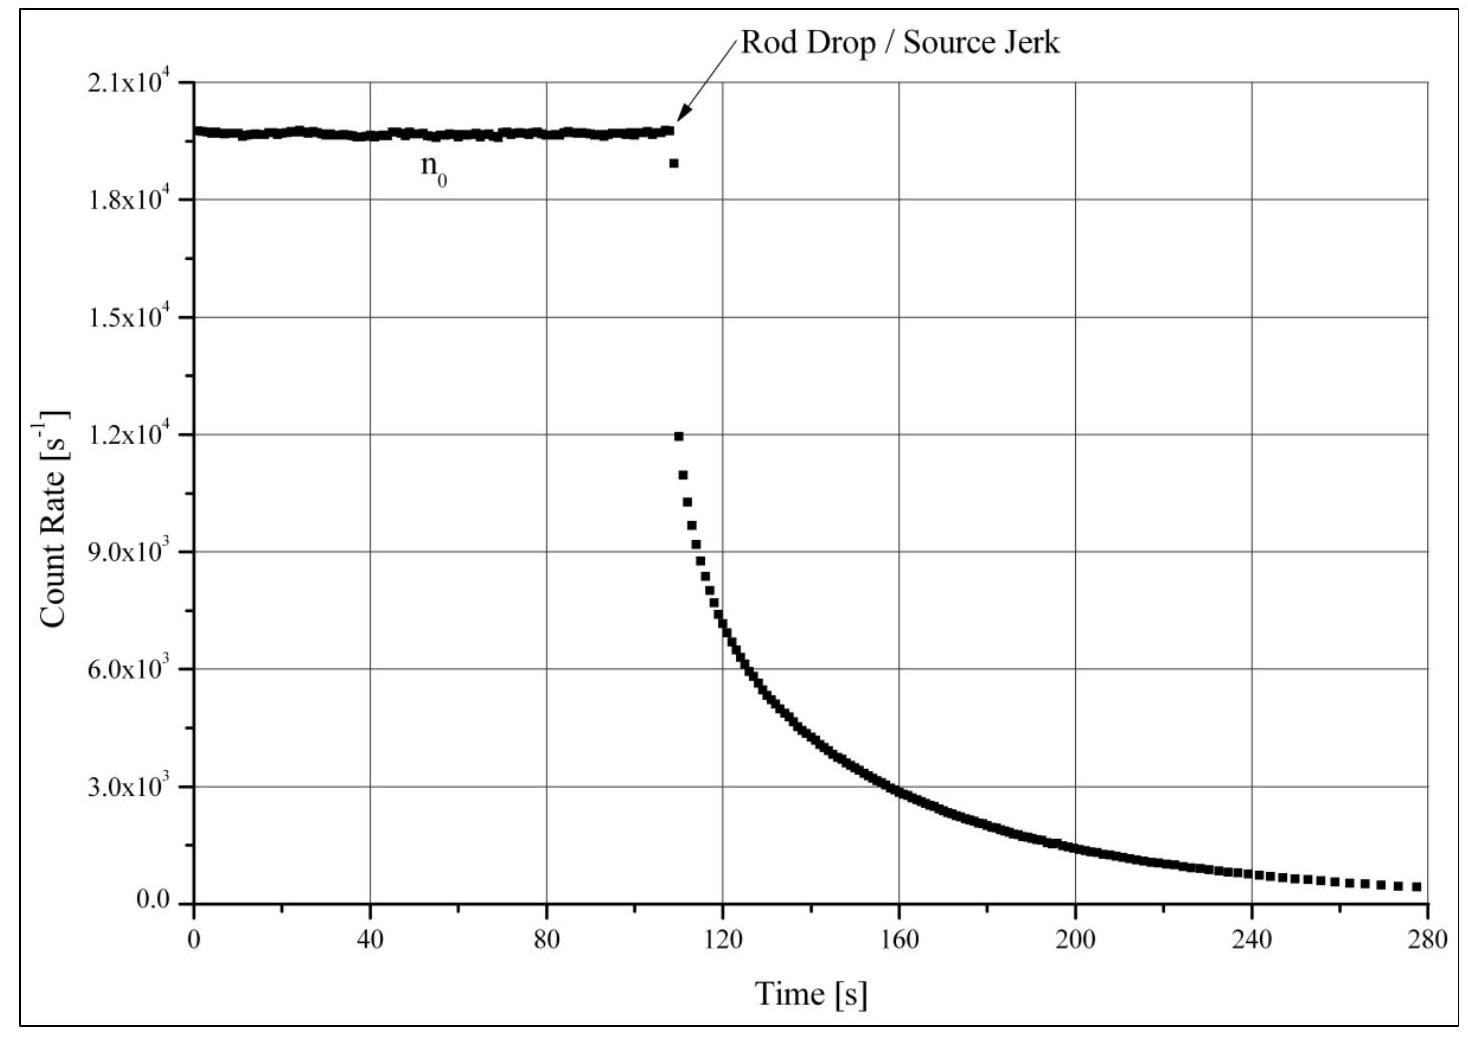
\includegraphics[max width=\textwidth]{2023_01_12_fb43672477d35ecded7eg-5}
\end{center}

Fig. 6.1 Detected neutron rate time evolution during the reactivity measurement by Rod Drop/Source Jerk method

The measurement of the reactivity by the Source Jerk method is done in the following manner:

\begin{enumerate}
  \item Insert the external neutron source into the core (usually done after the Rod Drop measurement).

  \item Wait for reactor stabilization.

  \item Determine the neutron rate $\mathrm{n}(0)$ before the source is removed from the core.

\end{enumerate}

\end{document}